\begin{frame}
\frametitle{Time your commands using the time command}
\begin{center}
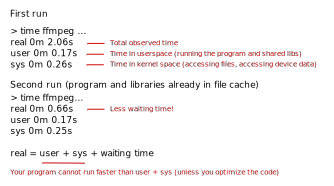
\includegraphics[height=0.7\textheight]{slides/boot-time-toolchain2/using-time-command.pdf}
\end{center}
This gives you the best time that can possibly be achieved (with the fastest storage).
\end{frame}

\setuplabframe {Trying a Thumb2 toolchain}
{
\begin{itemize}
\item Measure filesystem and \code{ffmpeg} binary size. Time
      the execution of the application.
\item Re-compile the root filesystem using a Thumb2 toolchain
\item Measure size and time again.
\end{itemize}
}


\begin{frame}
\frametitle{Lessons from labs: ARM vs Thumb2}
\begin{itemize}
\item Testcase: root filesystem with \code{ffmpeg} and associated
      libraries (from our training labs)
\item Compiled with gcc 7.4, generating {\em ARM} code:\\
      Total filesystem size: 3.79 MB\\
      \code{ffmpeg} size: 227 KB
\item Compiled with gcc 7.4, generating {\em Thumb2} code:\\
      Total filesystem size: 3.10 MB (-18 \%)\\
      \code{ffmpeg} size: 183 KB (-19 \%)
\item Performance aspect: performance apparently slightly improved with Thumb2
      (approximately less than 5 \%, but there are slight variations in measured
      execution time, for one run to another).
\end{itemize}
\end{frame}

\begin{frame}
\frametitle{Lessons from labs: musl vs uClibc}
{\em Tested while preparing the labs (too long to do this during the
class)}\\

Tried to replace {\em uClibc} by {\em musl} in our video player lab:
\begin{itemize}
   \item musl library size: 680 KB (size of the \code{tar} archive for \code{lib/})
   \item uClibc library size: 570 KB
   \item uClibc saves 110 KB (useful), but otherwise no other significant change
    in filesystem and code size. Not a surprise when the system is mostly filled
    with binaries relying on shared libraries.
\end{itemize}
We stuck to {\em uClibc}!
\end{frame}
